% !TeX spellcheck = en_US
\addsection{Components}{\skills/luck.png}

\iftoggle{printable}{\vspace{-\baselineskip}}{}

This guide provides a visual overview of all components included in every expansion. For detailed information, including exact quantities and images of each individual component, please refer to the Archon's official content guide.

\vspace*{-1em}
\begin{figure}[H]
  \centering
  \begin{subfigure}[t]{0.4\linewidth}
    \includegraphics[width=\linewidth]{\images/combat_board.png}
    \caption{\textbf{\pagelink{Combat}{Combat Board}}}
  \end{subfigure}
  ~
  \begin{subfigure}[t]{0.4\linewidth}
    \includegraphics[width=\linewidth]{\images/battlefield-alone.png}
    \caption{\textbf{Battlefield Board} \\\textit{(Battlefield Expansion)}}
  \end{subfigure}
\end{figure}
\vspace*{-1.5em}
\begin{figure}[H]
  \centering
  \begin{subfigure}[b]{0.16\linewidth}
    \centering
    \includegraphics[width=0.6\linewidth]{\images/initiative-bf.png}
    \caption{\textbf{Initiative Token} \textit{(Battlefield Expansion)}}
  \end{subfigure}
  ~
  \begin{subfigure}[b]{0.25\linewidth}
    \centering
    \includegraphics[width=\linewidth]{\images/map-tile-back.png}
    \caption{\textbf{\pagelink{Map}{Map Tile}}}
  \end{subfigure}
  ~
  \begin{subfigure}[b]{0.25\linewidth}
    \includegraphics[width=\linewidth]{\images/hero.png}
    \caption{\textbf{\pagelink{Herocard}{Hero Card}}}
  \end{subfigure}
  ~
  \begin{subfigure}[b]{0.25\linewidth}
    \includegraphics[width=\linewidth]{\images/town.png}
    \caption{\textbf{\pagelink{Town}{Town Board}}}
  \end{subfigure}
\end{figure}
\vspace*{-1.7em}
\begin{figure}[H]
  \centering
  \begin{subfigure}[t]{0.15\linewidth}
    \centering
    \includegraphics[width=0.8\linewidth]{\images/grail.png}
    \caption{\textbf{\pagelink{Grail}{Grail Token} \phantom{Population}}}
  \end{subfigure}
  \begin{subfigure}[t]{0.18\linewidth}
    \centering
    \includegraphics[width=\linewidth]{\images/gold-tokens.png}
    \caption{\textbf{\pagelink{Resources}{Gold Tokens}}}
  \end{subfigure}
  \begin{subfigure}[c]{0.12\linewidth}
    \centering
    \includegraphics[width=0.6\linewidth]{\images/building-materials-token.png}
    \caption{\textbf{\pagelink{Resources}{Building Materials}}}
  \end{subfigure}
  \begin{subfigure}[c]{0.12\linewidth}
    \centering
    \includegraphics[width=0.6\linewidth]{\images/valuables-token.png}
    \caption{\textbf{\pagelink{Resources}{Valuables Token}}}
  \end{subfigure}
  \begin{subfigure}[c]{0.12\linewidth}
    \centering
    \includegraphics[width=5em]{\images/build.png}
    \caption{\textbf{\pagelink{Town Actions}{Build Token}} \iftoggle{printable}{}{\phantom{Population}}}
  \end{subfigure}
  \begin{subfigure}[c]{0.13\linewidth}
    \centering
    \includegraphics[width=5em]{\images/population.png}
    \caption{\textbf{\pagelink{Town Actions}{Population Token}} \iftoggle{printable}{}{\phantom{Population}}}
  \end{subfigure}
  \begin{subfigure}[c]{0.12\linewidth}
    \centering
    \includegraphics[width=5em]{\images/spells.png}
    \caption{\textbf{\pagelink{Town Actions}{\mbox{Spell Book} Token}} \iftoggle{printable}{}{\phantom{Population}}}
  \end{subfigure}
\end{figure}
\vspace*{-3.5em}
\begin{figure}[H]
  \centering
  \begin{subfigure}[b]{0.2\linewidth}
    \begin{tikzpicture}
      \node at (0, 0) {\includegraphics[width=0.6\linewidth]{\images/morale-negative.png}};
      \node at (1, 0) {\includegraphics[width=0.6\linewidth]{\images/morale-positive.png}};
    \end{tikzpicture}
    \caption{\textbf{\pagelink{Morale}{Morale Token}}}
  \end{subfigure}
  \begin{subfigure}[b]{0.17\linewidth}
    \centering
    \includegraphics[width=4.5em]{\images/paralysis-defense.png}
    \caption{\textbf{\hyperlink{Paralysis}{Paralysis}/ \pagelink{Defend}{Defense} Token}}
  \end{subfigure}
  \begin{subfigure}[b]{0.1\linewidth}
    \centering
    \includegraphics[width=3em]{\images/damage-token.png}
    \caption{\textbf{\pagelink{combatround}{Damage Token}}}
  \end{subfigure}
  \begin{subfigure}[b]{0.15\linewidth}
    \centering
    \includegraphics[width=0.6\linewidth]{\images/movement-tokens.png}
    \caption{\textbf{\pagelink{Movement}{Movement Tokens}}}
  \end{subfigure}
  \begin{subfigure}[b]{0.15\linewidth}
    \centering
    \includegraphics[width=0.8\linewidth]{\images/faction-cubes.png}
    \caption{\textbf{Faction Cubes}}
  \end{subfigure}
  \begin{subfigure}[b]{0.15\linewidth}
    \centering
    \includegraphics[width=\linewidth]{\images/black-cubes.png}
    \caption{\textbf{Black Cubes}}
  \end{subfigure}
\end{figure}
\vspace*{-2em}
\begin{figure}[H]
  \centering
  \begin{subfigure}[b]{0.27\linewidth}
    \begin{tikzpicture}
      \node at (0, 0) {\includegraphics[width=0.45\linewidth]{\cards/morale-positive-back.png}};
      \node at (1.9, 0.1) {\includegraphics[width=0.45\linewidth]{\cards/morale-positive.png}};
    \end{tikzpicture}
    \caption{\textbf{Positive Morale Card} \textit{(Battlefield Expansion)}}
  \end{subfigure}
  \begin{subfigure}[b]{0.27\linewidth}
    \begin{tikzpicture}
      \node at (0, 0) {\includegraphics[width=0.45\linewidth]{\cards/morale-negative-back.png}};
      \node at (1.9, 0.1) {\includegraphics[width=0.45\linewidth]{\cards/morale-negative.png}};
    \end{tikzpicture}
    \caption{\textbf{Negative Morale Card} \textit{(Battlefield Expansion)}}
  \end{subfigure}
  \begin{subfigure}[b]{0.4\linewidth}
    \centering
    \includegraphics[width=\linewidth]{\images/hero-minis.png}
    \caption{\textbf{Hero Miniatures}}
  \end{subfigure}
\end{figure}
\vspace*{-2em}

\clearpage

\vspace*{-4em}
\begin{figure}[H]
  \centering
  \begin{subfigure}[t]{0.23\linewidth}
    \centering
    \begin{tikzpicture}
      \node at (0, 0) {\includegraphics[width=0.8\linewidth]{\cards/event-back.png}};
      \node at (0.7, 1.2) {\includegraphics[width=0.8\linewidth]{\cards/event.png}};
    \end{tikzpicture}
    \caption{\textbf{\pagelink{Events}{Event Card}}\\\textit{(Fortress Expansion)}}
  \end{subfigure}
  \begin{subfigure}[t]{0.25\linewidth}
    \centering
    \begin{tikzpicture}
      \node at (0, 0) {\includegraphics[width=0.7\linewidth]{\cards/astrolog-back.png}};
      \node at (0.7, 1.2) {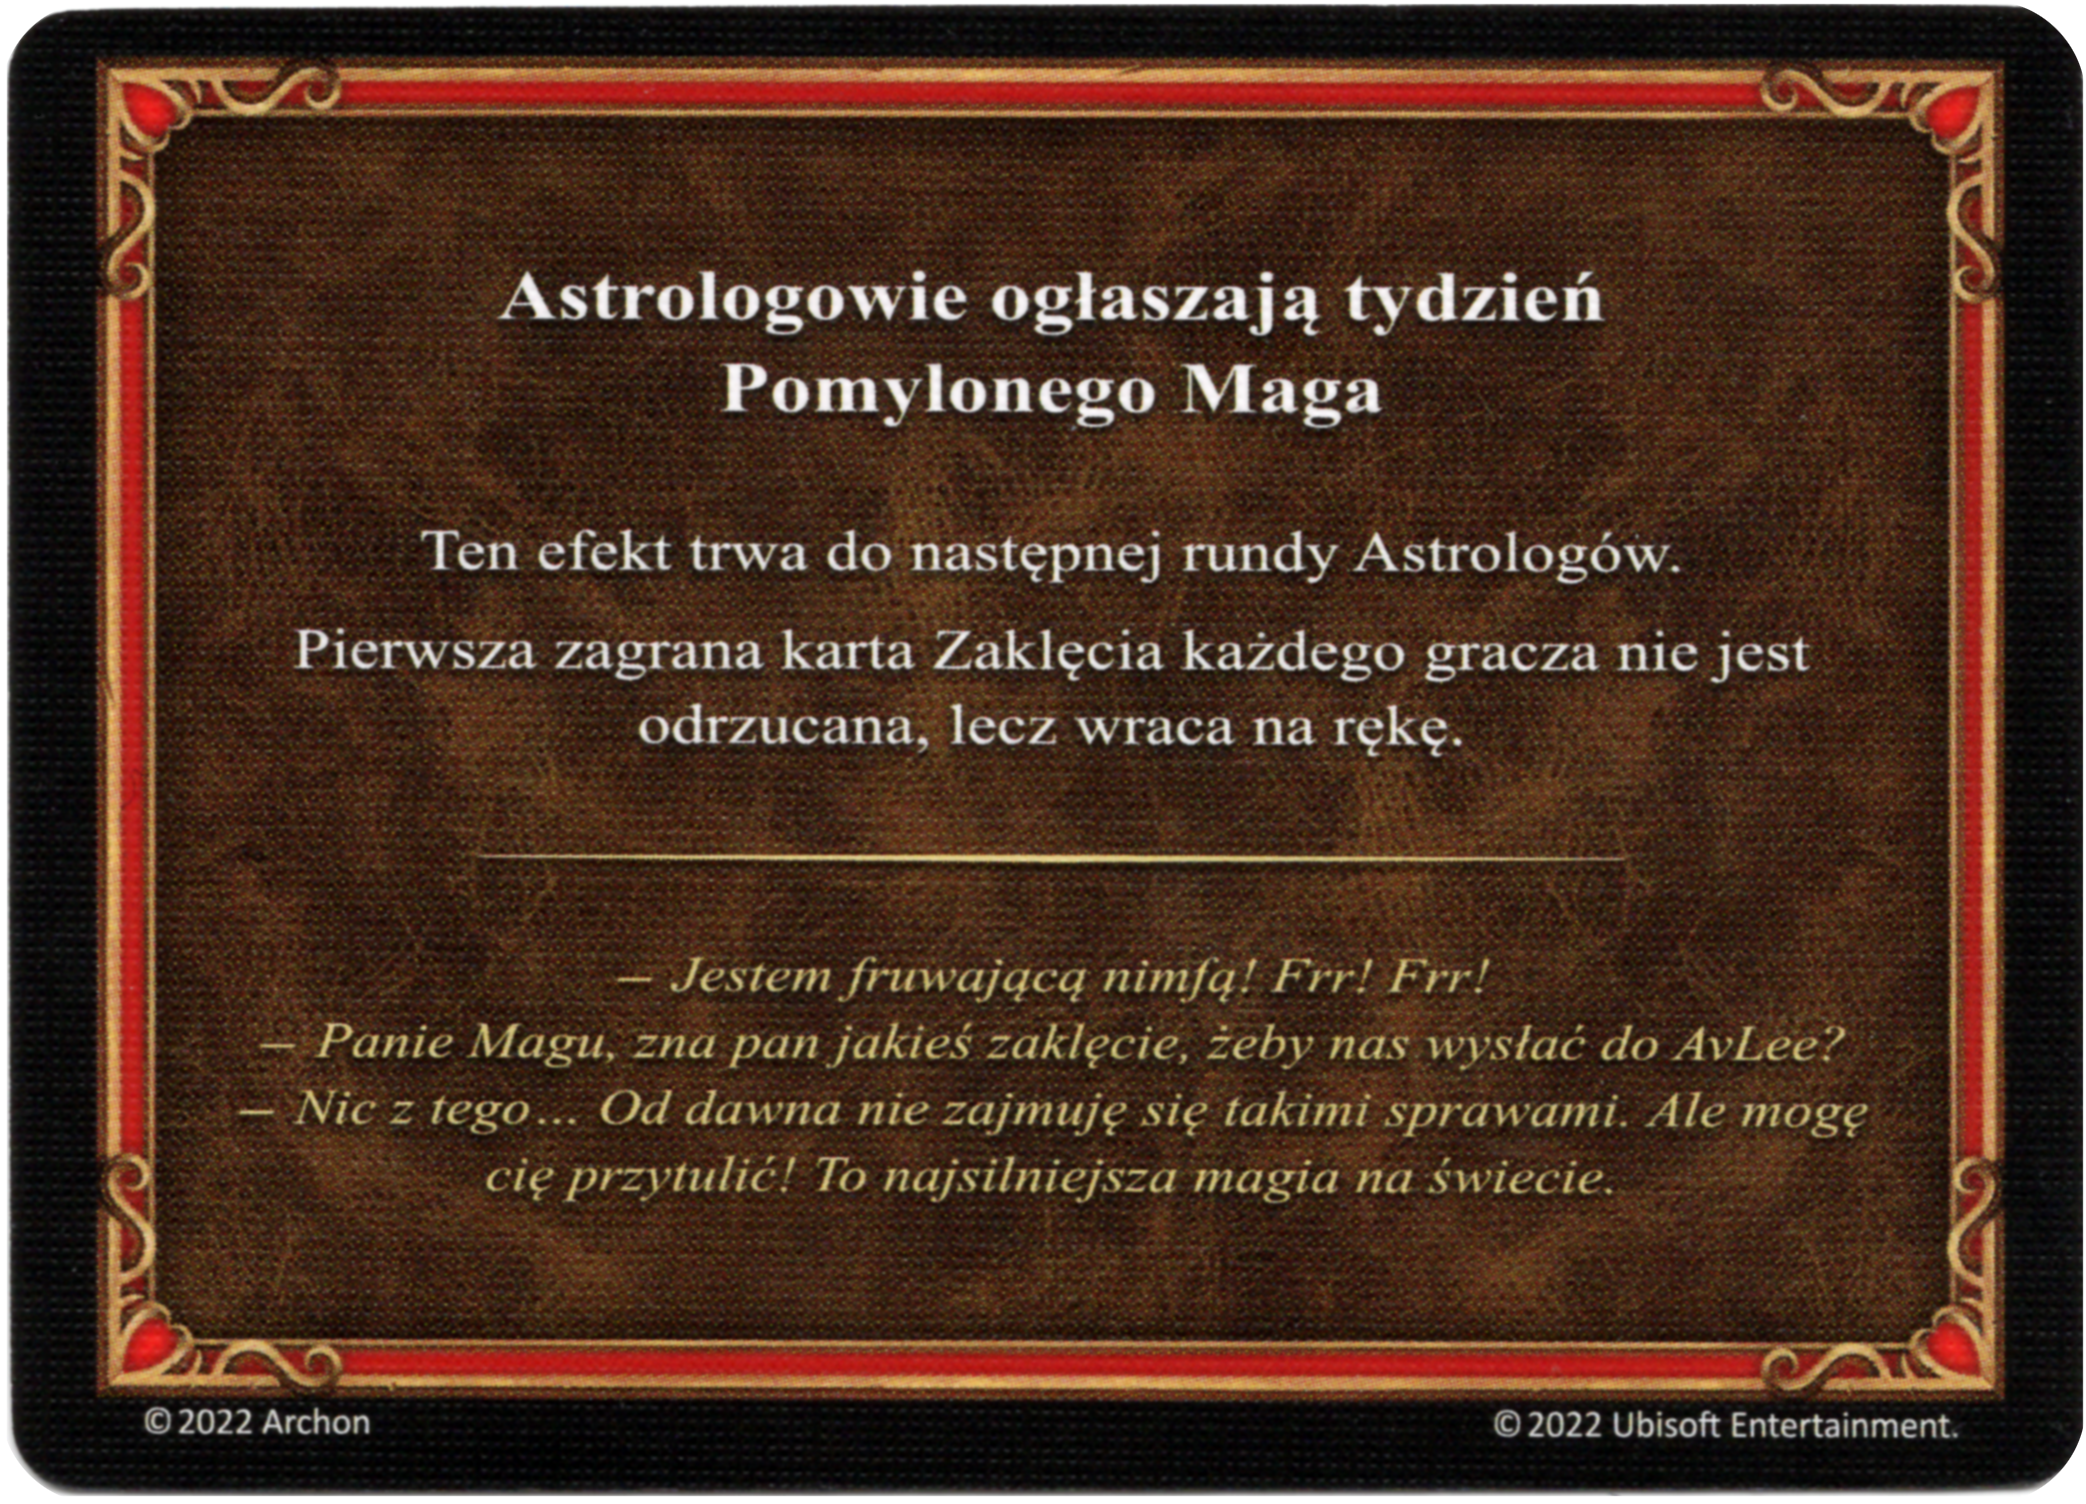
\includegraphics[width=0.7\linewidth]{\cards/astrolog.png}};
    \end{tikzpicture}
    \caption{\textbf{\pagelink{Rounds}{Astrologers Proclaim Card}}}
  \end{subfigure}
  \begin{subfigure}[t]{0.23\linewidth}
    \centering
    \includegraphics[width=\linewidth]{\cards/aiback.png}
    \caption{\textbf{\pagelink{AIrules}{AI Card}}}
  \end{subfigure}
  \begin{subfigure}[t]{0.25\linewidth}
    \centering
    \includegraphics[width=\linewidth]{\cards/adventure.png}
    \caption{\textbf{Adventure Card} \textit{(Battlefield Expansion)}}
  \end{subfigure}
\end{figure}
\vspace*{-2em}
\begin{figure}[H]
  \centering
  \begin{subfigure}[t]{0.23\linewidth}
    \centering
    \begin{tikzpicture}
      \node at (0, 0) {\includegraphics[width=0.6\linewidth]{\cards/mmback.png}};
      \node at (1.5, 0.1) {\includegraphics[width=0.6\linewidth]{\cards/necromancy_card.png}};
    \end{tikzpicture}
    \caption{\textbf{\pagelink{Ability}{Ability Card}}}
  \end{subfigure}
  \begin{subfigure}[t]{0.23\linewidth}
    \centering
    \begin{tikzpicture}
      \node at (0, 0) {\includegraphics[width=0.6\linewidth]{\cards/mmback.png}};
      \node at (1.5, 0.1) {\includegraphics[width=0.6\linewidth]{\cards/artifact-front.png}};
    \end{tikzpicture}
    \caption{\textbf{\pagelink{Artifact}{Artifact Card}}}
  \end{subfigure}
  \begin{subfigure}[t]{0.23\linewidth}
    \centering
    \begin{tikzpicture}
      \node at (0, 0) {\includegraphics[width=0.6\linewidth]{\cards/mmback.png}};
      \node at (1.5, 0.1) {\includegraphics[width=0.6\linewidth]{\cards/spell.png}};
    \end{tikzpicture}
    \caption{\textbf{\pagelink{spells}{Spell Card}}}
  \end{subfigure}
\end{figure}
\vspace*{-2em}
\begin{figure}[H]
  \centering
  \begin{subfigure}[t]{0.23\linewidth}
    \centering
    \begin{tikzpicture}
      \node at (0, 0) {\includegraphics[width=0.6\linewidth]{\cards/mmback.png}};
      \node at (1.5, 0.1) {\includegraphics[width=0.6\linewidth]{\cards/war_machine.png}};
    \end{tikzpicture}
    \caption{\textbf{\pagelink{War Machines}{War Machine Card}} \textit{(Rampart Expansion)}}
  \end{subfigure}
  \begin{subfigure}[t]{0.23\linewidth}
    \centering
    \begin{tikzpicture}
      \node at (0, 0) {\includegraphics[width=0.6\linewidth]{\cards/mmback.png}};
      \node at (1.5, 0.1) {\includegraphics[width=0.6\linewidth]{\cards/specialty.png}};
    \end{tikzpicture}
    \caption{\textbf{\pagelink{Specialty}{Hero Specialty Card}}}
  \end{subfigure}
  \begin{subfigure}[t]{0.23\linewidth}
    \centering
    \begin{tikzpicture}
      \node at (0, 0) {\includegraphics[width=0.6\linewidth]{\cards/mmback.png}};
      \node at (1.5, 0.1) {\includegraphics[width=0.6\linewidth]{\cards/statistic.png}};
    \end{tikzpicture}
    \caption{\textbf{\pagelink{Statistic}{Statistic Card}}}
  \end{subfigure}
  \begin{subfigure}[t]{0.23\linewidth}
    \centering
    \begin{tikzpicture}
      \node at (0, 0) {\includegraphics[width=0.6\linewidth]{\cards/mmback.png}};
      \node at (1.5, 0.1) {\includegraphics[width=0.6\linewidth]{\cards/empowered_statistic.png}};
    \end{tikzpicture}
    \caption{\textbf{\pagelink{Empowered Statistic}{Empowered Statistic Card}} \textit{(Inferno Expansion)}}
  \end{subfigure}
\end{figure}
\vspace*{\iftoggle{printable}{-2em}{-3em}}
\begin{figure}[H]
  \centering
  \begin{subfigure}[t]{0.23\linewidth}
    \centering
    \begin{tikzpicture}
      \node at (0, 0) {\includegraphics[width=0.6\linewidth]{\cards/neutral-back.png}};
      \node at (1.5, 0.1) {\includegraphics[width=0.6\linewidth]{\cards/neutral-front.png}};
    \end{tikzpicture}
    \caption{\textbf{\pagelink{Neutral Units}{Neutral Unit Card}}}
  \end{subfigure}
  ~
  \begin{subfigure}[t]{0.23\linewidth}
    \centering
    \begin{tikzpicture}
      \node at (0, 0) {\includegraphics[width=0.6\linewidth]{\cards/unit-pack.png}};
      \node at (1.5, 0.1) {\includegraphics[width=0.6\linewidth]{\cards/unit-few.png}};
    \end{tikzpicture}
    \caption{\textbf{\pagelink{Units}{Faction Unit Card}}}
  \end{subfigure}
  ~
  \begin{subfigure}[t]{0.23\linewidth}
    \centering
    \begin{tikzpicture}
      \node at (0, 0) {\includegraphics[width=0.6\linewidth]{\cards/arrow_tower_back.png}};
      \node at (1.5, 0.1) {\includegraphics[width=0.6\linewidth]{\cards/arrow_tower.png}};
    \end{tikzpicture}
    \caption{\textbf{\pagelink{Walls}{Arrow Tower Card}}}
  \end{subfigure}
  ~
  \begin{subfigure}[t]{0.23\linewidth}
    \centering
    \includegraphics[width=\linewidth]{\cards/gate.png}
    \caption{\textbf{\pagelink{Walls}{Gate, Walls Cards}}}
  \end{subfigure}
\end{figure}

\vspace*{-2em}
\columnratio{0.4}
\begin{paracol}{2}
\begin{figure}[H]
  \centering
  \begin{subfigure}[b]{0.3\linewidth}
    \centering
    \includegraphics[width=0.7\linewidth]{\images/attack_die.png}
    \caption{\textbf{Attack Dice}}
  \end{subfigure}
  \begin{subfigure}[b]{0.3\linewidth}
    \centering
    \includegraphics[width=\linewidth]{\images/treasure_die.png}
    \caption{\textbf{Treasure Dice}}
  \end{subfigure}
  \begin{subfigure}[b]{0.3\linewidth}
    \centering
    \includegraphics[width=0.8\linewidth]{\images/resource_die.png}
    \caption{\textbf{Resource Dice}}
  \end{subfigure}
\end{figure}
\vspace*{-2em}
\begin{figure}[H]
  \centering
  \begin{subfigure}[b]{\iftoggle{printable}{0.8\linewidth}{\linewidth}}
    \centering
    \includegraphics[width=0.8\linewidth]{\images/round-tracker.png}
    \caption{\textbf{\pagelink{Rounds}{Round Tracker}}}
  \end{subfigure}
\end{figure}
\vspace*{-1em}
\switchcolumn
\begin{figure}[H]
  \vspace*{1em}
  \centering
  \begin{subfigure}[b]{\iftoggle{printable}{0.8\linewidth}{\linewidth}}
    \centering
    \includegraphics[width=\linewidth]{\images/battlefield-obstacles.png}
    \caption{\textbf{Obstacles} \textit{(Battlefield Expansion)}}
  \end{subfigure}
\end{figure}
\end{paracol}
